
\chapter{Árboles}

\index{árbol} \index{nodo} \index{nodo de un árbol} \index{carga}
\index{referencia incrustada} \index{árbol binario}

Como las listas enlazadas, los árboles están compuestos de nodos.
Una clase muy común es el \textbf{árbol binario}, en el que cada nodo
contiene una referencia a otros dos nodos (posiblemente nulas). Estas
referencias se denominan los subárboles izquierdo y derecho. Como
los nodos de las listas, los nodos de los árboles también contienen
una carga. Un diagrama de estados para los árboles luce así:

\label{tree} \beforefig \centerline{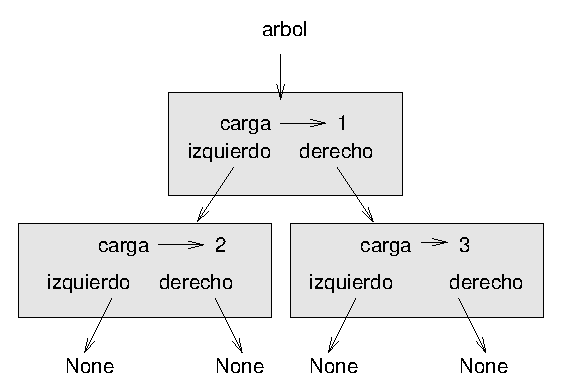
\includegraphics{illustrations/tree1}}
\afterfig

Para evitar el caos en las figuras, a menudo omitimos los valores
\texttt{None}.

El inicio del árbol (al nodo al que \texttt{árbol} se refiere) se
denomina \textbf{raíz}. Para conservar la metáfora con los árboles,
los otros nodos se denominan ramas, y los nodos que tienen referencias
nulas se llaman \textbf{hojas}. Parece extraño el dibujo con la raíz
en la parte superior y las hojas en la inferior, pero esto es sólo
el principio.

\index{nodo raíz} \index{nodo hoja} \index{nodo padre} \index{nodo hijo}
\index{nivel}

Los científicos de la computación también usan otra metáfora—el árbol
genealógico. El nodo raíz se denomina \textbf{padre} y los nodos a
los que se refiere \textbf{hijos}, los nodos que tienen el mismo padre
se denominan \textbf{hermanos}.

Finalmente, hay un vocabulario geométrico para referirse a los árboles.
Ya mencionamos la distinción entre izquierda y derecha, también se
acostumbra diferenciar entre ``arriba'' (hacia el padre/raíz) y
``abajo'' (hacia los hijos/hojas). Además, todos los nodos que están
a una misma distancia de la raíz comprenden un \textbf{nivel}.

Probablemente no necesitemos estas metáforas para describir los árboles,
pero se usan extensivamente.

Como las listas enlazadas, los árboles son estructuras de datos recursivas
ya que su definición es recursiva.

\index{estructuras de datos recursivas} \index{estructuras de datos!recursivas}
\begin{quote}
Un árbol es:

\begin{itemize}
\item el árbol vacío, representado por \texttt{None}, o
\item Un nodo que contiene una referencia a un objeto y referencias a otros
aŕboles.
\end{itemize}
\end{quote}
\index{árbol!vacío}

\section{Construyendo árboles}

El proceso de construir un árbol es similar al de una lista enlazada.
La llamada al constructor arma un árbol con un solo nodo.

\beforeverb 
\begin{pythoncode}
class arbol:
  def __init__(self, carga, izquierdo=None, derecho=None):
    self.carga = carga
    self.izquierdo  = izquierdo
    self.derecho = derecho

  def __str__(self):
    return str(self.carga)
\end{pythoncode}
\afterverb La \texttt{carga} puede tener cualquier tipo, pero los
parámetros \texttt{izquierdo} y \texttt{derecho} deben ser nodos.
En \texttt{\_\_init\_\_}, \texttt{izquierdo} y \texttt{derecho} son
opcionales; su valor por defecto es \texttt{None}. Imprimir un nodo
equivale a imprimir su carga.

Una forma de construir un árbol es de abajo hacia arriba. Primero
se construyen los nodos hijos:

\beforeverb 
\begin{pythoncode}
izquierdo = arbol(2)
derecho = arbol(3)
\end{pythoncode}
\afterverb Ahora se crea el padre y se enlazan los hijos:

\beforeverb 
\begin{pythoncode}
arbol = arbol(1, izquierdo, derecho);
\end{pythoncode}
\afterverb Podemos escribir esto de una manera más compacta anidando
los llamados:

\beforeverb 
\begin{pyconcode}
>>> arbol = arbol(1, arbol(2), arbol(3))
\end{pyconcode}
\afterverb Con las dos formas se obtiene como resultado el árbol
que ilustramos al principio del capítulo.

\section{Recorridos sobre árboles}

\index{árbol!recorrido} \index{recorrer} \index{recursión}

Cada vez que se encuentre con una nueva estructura de datos su primera
pregunta debería ser, ``¿Cóomo la recorro?''. La forma más natural
de recorrer un árbol es recursiva. Si el árbol contiene números enteros
en la carga, esta función calcula su suma :

\beforeverb 
\begin{pythoncode}
def total(arbol):
  if arbol == None: 
     return 0
  else:
     return total(arbol.izquierdo) + total(arbol.derecho) 
            + arbol.carga
\end{pythoncode}
\afterverb El caso base se da cuando el argumento es el árbol vacío,
que no tiene carga, así que la suma se define como 0. El paso recursivo
realiza dos llamados recursivos para encontrar la suma de los árboles
hijos, cuando finalizan, se suma a estos valores la carga del padre.

\section{Árboles de expresiones}

\index{árbol!expresión} \index{árbol para una expresión} \index{postfija}
\index{infija} \index{operador binario} \index{operador!binario}

Un árbol representa naturalmente la estructura de una expresión. Además,
lo puede realizar sin ninguna ambigüedad. Por ejemplo, la expresión
infija \texttt{1 + 2 {*} 3} es ambigua a menos que se establezca que
la multiplicación se debe realizar antes que la suma.

Este árbol representa la misma expresión:

\beforefig \centerline{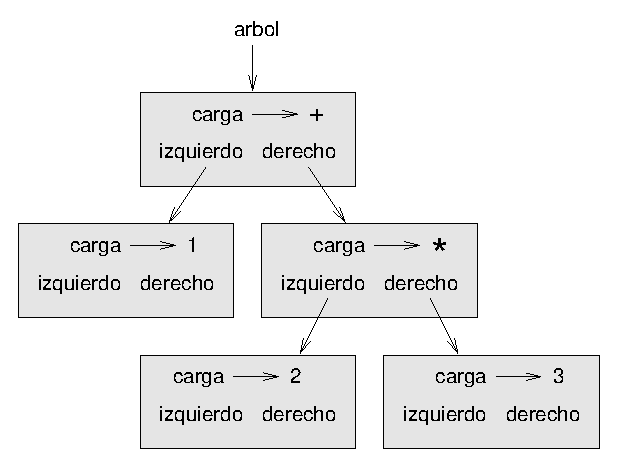
\includegraphics{illustrations/tree2}}
\afterfig

Los nodos de un árbol para una expresión pueden ser operandos como
\texttt{1} y \texttt{2}, también operadores como \texttt{+} y \texttt{{*}}.
Los operandos deben ser nodos hoja; y los nodos que contienen operadores
tienen referencias a sus operandos. Todos estos operadores son \textbf{binarios},
así que solamente tienen dos operandos.

Un árbol como el siguiente representa la figura anterior:

\beforeverb 
\begin{pyconcode}
>>> arbol = arbol('+', arbol(1), 
                       arbol('*', arbol(2), arbol(3)))
\end{pyconcode}
\afterverb Observando la figura no hay ninguna duda sobre el orden
de las operaciones; la multiplicación ocurre primero para que se calcule
el segundo operando de la suma.

Los árboles de expresiones tienen muchos usos. El ejemplo de este
capítulo utiliza árboles para traducir expresiones entre las notaciones
postfija, prefija, e infija. Árboles similares se usan en los compiladores
para analizar sintácticamente, optimizar y traducir programas.

\section{Recorrido en árboles}

\index{árbol!recorrido} \index{recorrido} \index{recursión} \index{Preorden}
\index{Postorden} \index{EnOrden}

Podemos recorrer un árbol de expresiones e imprimir el contenido de
la siguiente forma:

\beforeverb 
\begin{pythoncode}
def imprimirarbol(arbol):
  if arbol == None: 
     return
  print(arbol.carga),
  imprimirarbol(arbol.izquierdo)
  imprimirarbol(arbol.derecho)
\end{pythoncode}
\afterverb \index{Preorden} \index{prefija}

En otras palabras, para imprimir un árbol, primero se imprime el contenido
(carga) de la raíz, luego todo el subárbol izquierdo, y a continuación
todo el subárbol derecho. Este recorrido se denomina \textbf{preorden},
porque el contenido de la raíz se despliega {\em antes} que el
contenido de los hijos. Para el ejemplo anterior, la salida es:

\beforeverb 
\begin{pyconcode}
>>> arbol = arbol('+', arbol(1), 
                       arbol('*', arbol(2), arbol(3)))
>>> imprimirarbol(arbol)
+ 1 * 2 3
\end{pyconcode}
\afterverb Esta notación diferente a la infija y a la postfija, se
denomina \textbf{prefija}, porque los operadores aparecen antes que
sus operandos.

Usted puede sospechar que si se recorre el árbol de una forma distinta
se obtiene otra notación. Por ejemplo si se despliegan los dos subárboles
primero y a continuación el nodo raíz, se obtiene

\beforeverb 
\begin{pythoncode}
def imprimirarbolPostorden(arbol):
  if arbol == None: 
     return
  else 
     imprimirarbolPostorden(arbol.izquierdo)
     imprimirarbolPostorden(arbol.derecho)
     print(arbol.carga),
\end{pythoncode}
\afterverb \index{postorden} \index{en orden} El resultado, \texttt{1
2 3 {*} +}, está en notación postfija!. Por esta razón este recorrido
se denomina \textbf{postorden}.

Finalmente, para recorrer el árbol \textbf{en orden}, se imprime el
árbol izquierdo, luego la raíz y, por último, el árbol derecho:

\beforeverb 
\begin{pythoncode}
def imprimirabolEnOrden(árbol):
  if arbol == None: 
     return
  imprimirabolEnOrden(arbol.izquierdo)
  print(arbol.carga),
  imprimirabolEnOrden(arbol.derecho)
\end{pythoncode}
\afterverb El resultado es \texttt{1 + 2 {*} 3}, la expresión en
notación infija.

Por precisión debemos anotar que hemos omitido una complicación importante.
Algunas veces cuando escribimos una expresión infija, tenemos que
usar paréntesis para preservar el orden de las operaciones. Así que
un recorrido en orden no es suficiente en todos los casos para generar
una expresión infija.

Sin embargo, con unas mejoras adicionales, los árboles de expresiones
y los tres recorridos recursivos proporcionan una forma general de
traducir expresiones de un formato al otro.
\begin{quote}
{\em Como ejercicio, modifique \texttt{imprimirarbolEnOrden} para
que despliegue paréntesis alrededor de cada operador y pareja de operandos.
¿La salida es correcta e inequívoca? ¿Siempre son necesarios los paréntesis?
} 
\end{quote}
Si realizamos un recorrido en orden y llevamos pista del nivel en
el que vamos podemos generar una representación gráfica del árbol:

\beforeverb 
\begin{pythoncode}
def imprimirarbolSangrado(arbol, nivel=0):
  if arbol == None: 
     return
  imprimirarbolSangrado(arbol.derecho, nivel+1)
  print('  '*nivel + str(arbol.carga))
  imprimirarbolSangrado(arbol.izquierdo, nivel+1)
\end{pythoncode}
\afterverb El parámetro \texttt{nivel} lleva el nivel actual. Por
defecto es 0. Cada vez que hacemos un llamado recursivo pasamos \texttt{nivel+1},
porque el nivel de los hijos siempre es uno más del nivel del padre.
Cada objeto se sangra o indenta con dos espacios por nivel. El resultado
para el árbol de ejemplo es:

\beforeverb 
\begin{pyconcode}
>>> imprimirarbolSangrado(arbol)
    3
  *
    2
+
  1
\end{pyconcode}
\afterverb Si rota el libro 90 grados en el sentido de las manecillas
del reloj verá una forma simplificada del dibujo al principio del
capítulo.

\section{Construyendo un árbol para una expresión}

\index{árbol para una expresión} \index{árbol!expresión} \index{análisis sintáctico}
\index{lexema}

En esta sección, analizaremos sintácticamente expresiones infijas
para construir su respectivo árbol de expresión. Por ejemplo, la expresión
\texttt{(3+7){*}9} se representa con el siguiente árbol:

\beforefig \centerline{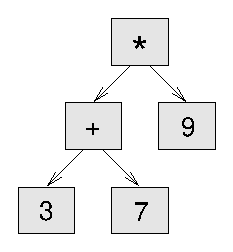
\includegraphics{illustrations/tree3}}
\afterfig

Note que hemos simplificado el diagrama ocultando los nombres de los
atributos.

El análisis sintáctico se hará sobre expresiones que incluyan números,
paréntesis, y los operadores \texttt{+} y \texttt{{*}}. Asumimos que
la cadena de entrada ha sido separada en una lista de lexemas; por
ejemplo, para \texttt{(3+7){*}9} la lista de lexemas es:

\beforeverb 
\begin{pythoncode}
['(', 3, '+', 7, ')', '*', 9, 'fin']
\end{pythoncode}
\afterverb La cadena \texttt{fin} sirve para prevenir que el analizador
sintáctico siga leyendo más allá del final de la lista.
\begin{quote}
{\em Como ejercicio escriba una función que reciba una cadena de
texto con una expresión y retorne la lista de lexemas (con la cadena
\texttt{fin} al final).} 
\end{quote}
La primera función que escribiremos es \texttt{obtenerLexema}, que
toma una lista de lexemas y un lexema esperado como parámetros. Compara
el lexema esperado con el primero de la lista: si son iguales, elimina
el lexema de la lista y retorna True, si no son iguales, retorna False:

\beforeverb 
\begin{pythoncode}
def obtenerLexema(listaLexemas, esperado):
  if listaLexemas[0] == esperado:
    del listaLexemas[0]
    return 1
  else:
    return 0
\end{pythoncode}
\afterverb Como \texttt{listaLexemas} se refiere a un objeto mutable,
los cambios que hacemos son visibles en cualquier otra parte del programa
que tenga una referencia a la lista.

La siguiente función, \texttt{obtenerNumero}, acepta operandos. Si
el siguiente lexema en \texttt{listaLexemas} es un número, \texttt{obtenerNumero}
lo elimina y retorna un nodo hoja cuya carga será el número; si no
es un número retorna \texttt{None}.

\beforeverb 
\begin{pythoncode}
def obtenerNumero(listaLexemas):
  x = listaLexemas[0]
  if type(x) != type(0): 
     return None
  del listaLexemas[0]
  return arbol (x, None, None)
\end{pythoncode}
\afterverb Probemos a \texttt{obtenerNumero} con una lista pequeña
de números. Después del llamado, imprimimos el árbol resultante y
lo que queda de la lista:

\beforeverb 
\begin{pyconcode}
>>> listaLexemas = [9, 11, 'fin']
>>> x = obtenerNumero(listaLexemas)
>>> imprimirarbolPostorden(x)
9
>>> print(listaLexemas)
[11, 'fin']
\end{pyconcode}
\afterverb El siguiente método que necesitamos es \texttt{obtenerProducto},
que construye un árbol de expresión para productos. Un producto sencillo
tiene dos números como operandos, como en \texttt{3 {*} 7}.

\beforeverb 
\begin{pythoncode}
def obtenerProducto(listaLexemas):
  a = obtenerNumero(listaLexemas)
  if obtenerLexema(listaLexemas, '*'):
    b = obtenerNumero(listaLexemas)
    return árbol ('*', a, b)
  else:
    return a
\end{pythoncode}
\afterverb Asumiendo que \texttt{obtenerNumero} retorna un árbol,
le asignamos el primer operando a \texttt{a}. Si el siguiente carácter
es \texttt{{*}}, obtenemos el segundo número y construimos un árbol
de expresión con \texttt{a}, \texttt{b}, y el operador.

Si el siguiente carácter es cualquier otro, retornamos el nodo hoja
con \texttt{a}. Aquí hay dos ejemplos:

\beforeverb 
\begin{pyconcode}
>>> listaLexemas = [9, '*', 11, 'fin']
>>> arbol = obtenerProducto(listaLexemas)
>>> imprimirarbolPostorden(árbol)
9 11 *
\end{pyconcode}
\afterverb

\beforeverb 
\begin{pyconcode}
>>> listaLexemas = [9, '+', 11, 'fin']
>>> arbol = obtenerProducto(listaLexemas)
>>> imprimirarbolPostorden(arbol)
9
\end{pyconcode}
\afterverb El segundo ejemplo implica que consideramos que un solo
operando sea tratado como una clase de producto. Esta definición de
``producto'' es contraintuitiva, pero resulta ser muy provechosa.

Ahora, tenemos que manejar los productos compuestos, como \texttt{3
{*} 5 {*} 13}. Esta expresión es un producto de productos, vista así:
\texttt{3 {*} (5 {*} 13)}. El árbol resultante es:

\beforefig \centerline{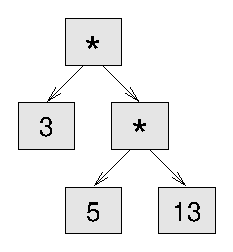
\includegraphics{illustrations/tree4}}
\afterfig

Con un pequeño cambio en \texttt{obtenerProducto}, podemos analizar
un producto arbitrariamente largo:

\beforeverb 
\begin{pythoncode}
def obtenerProducto(listaLexemas):
  a = obtenerNumero(listaLexemas)
  if obtenerLexema(listaLexemas, '*'):
    b = obtenerProducto(listaLexemas)   # esta línea cambió
    return arbol ('*', a, b)
  else:
    return a
\end{pythoncode}
\afterverb En otras palabras, un producto puede ser un árbol singular
o un árbol con \texttt{{*}} en la raíz, un número en el subárbol izquierdo,
y un producto en el subárbol derecho.

Esta clase de definición recursiva debería empezar a ser familiar.

\index{producto} \index{definición!recursiva} \index{definición recursiva}

Probemos la nueva versión con un producto compuesto:

\beforeverb 
\begin{pyconcode}
>>> listaLexemas = [2, '*', 3, '*', 5 , '*', 7, 'fin']
>>> arbol = obtenerProducto(listaLexemas)
>>> imprimirarbolPostorden(arbol)
2 3 5 7 * * *
\end{pyconcode}
\afterverb Ahora, agregaremos la posibilidad de analizar sumas. Otra
vez daremos una definición contraintuitiva a la ``suma.'' Una suma
puede ser un árbol con \texttt{+} en la raíz, un producto en el subárbol
izquierdo y una suma en el subárbol derecho. O, una suma puede ser
sólo un producto.

\index{suma}

Si usted analiza esta definición encontrará que tiene una propiedad
muy bonita: podemos representar cualquier expresión (sin paréntesis)
como una suma de productos. Esta propiedad es el fundamento de nuestro
algoritmo de análisis sintáctico.

\texttt{obtenerSuma} intenta construir un árbol con un producto en
izquierdo y una suma en derecho. Pero si no encuentra un \texttt{+},
solamente construye un producto.

\beforeverb 
\begin{pythoncode}
def obtenerSuma(listaLexemas):
  a = obtenerProducto(listaLexemas)
  if obtenerLexema(listaLexemas, '+'):
    b = obtenerSuma(listaLexemas)
    return arbol ('+', a, b)
  else:
    return a
\end{pythoncode}
\afterverb Probemos con \texttt{9 {*} 11 + 5 {*} 7}:

\beforeverb 
\begin{pyconcode}
>>> listaLexemas = [9, '*', 11, '+', 5, '*', 7, 'fin']
>>> arbol = obtenerSuma(listaLexemas)
>>> imprimirarbolPostorden(árbol)
9 11 * 5 7 * +
\end{pyconcode}
\afterverb Casi terminamos, pero todavía faltan los paréntesis. En
cualquier posición de una expresión donde podamos encontrar un número
puede también haber una suma completa cerrada entre paréntesis. Necesitamos
modificar \texttt{obtenerNumero} para que sea capaz de manejar \textbf{subexpresiones}:

\index{subexpresión}

\beforeverb 
\begin{pythoncode}
def obtenerNumero(listaLexemas):
  if obtenerLexema(listaLexemas, '('):
    # obtiene la subexpresión
    x = obtenerSuma(listaLexemas)  
    # elimina los paréntesis
    obtenerLexema(listaLexemas, ')') 
    return x
  else:
    x = listaLexemas[0]
    if type(x) != type(0): 
       return None
    listaLexemas[0:1] = []
    return árbol (x, None, None)    
\end{pythoncode}
\afterverb Probemos esto con \texttt{9 {*} (11 + 5) {*} 7}:

\beforeverb 
\begin{pyconcode}
>>> listaLexemas = [9, '*', '(', 11, '+', 5, ')','*', 7, 
'fin']
>>> arbol = obtenerSuma(listaLexemas)
>>> imprimirarbolPostorden(arbol)
9 11 5 + 7 * *
\end{pyconcode}
\afterverb %\adjustpage{-2}%\pagebreak

El analizador manejó los paréntesis correctamente, la suma se hace
antes que la multiplicación.

En la versión final del programa, sería bueno nombrar a \texttt{obtenerNumero}
con un rol más descriptivo.

\section{Manejo de errores}

\index{manejo de errores} \index{errores!manejo de}

En todo momento hemos asumido que las expresiones están bien formadas.
Por ejemplo, cuando llegamos al final de una subexpresión, asumimos
que el siguiente carácter es un paréntesis derecho. Si hay un error
y el siguiente carácter es algo distinto debemos manejar esta situación.

\beforeverb 
\begin{pythoncode}
def obtenerNumero(listaLexemas):
  if obtenerLexema(listaLexemas, '('):
    x = obtenerSuma(listaLexemas)       
    if not obtenerLexema(listaLexemas, ')'):
      raise 'ErrorExpresionMalFormada', 'falta paréntesis'
    return x
  else:
    # el resto del código se omite
\end{pythoncode}
\afterverb La sentencia \texttt{raise} crea una excepción. En este
caso creamos una nueva clase de excepción llamada \texttt{ErrorExpresionMalFormada}.
Si la función que llamó a \texttt{obtenerNumero}, o una de las funciones
en la traza que causante de su llamado maneja la excepción, el programa
puede continuar. De otra forma, Python imprimirá un mensaje de error
y abortará la ejecución.
\begin{quote}
{\em Como ejercicio, encuentre otros lugares donde pueden ocurrir
errores de este tipo y agregue sentencias \texttt{raise} apropiadas.
Pruebe su código con expresiones mal formadas.} 
\end{quote}

\section{El árbol de animales}

\index{juego de animales} \index{juego!de animales} \index{base de conocimiento}

En esta sección desarrollaremos un pequeño programa que usa un árbol
para representar una base de conocimiento.

El programa interactúa con el usuario para crear un árbol de preguntas
y nombres de animales. Aquí hay una ejecución de ejemplo:

\adjustpage{-3} %\pagebreak

\beforeverb 
\begin{pythoncode}
¿Esta pensando en un animal? s
¿Es un pájaro? n
¿Cual es el nombre del animal? perro
¿Que pregunta permite distinguir entre un perro 
y un pájaro? Puede volar
¿Si el animal fuera perro la respuesta sería? n

¿Esta pensando en un animal? s
¿Puede volar? n
¿Es un perro? n
¿Cual es el nombre del animal? gato
¿Que pregunta permite distinguir un gato 
de un perro? Ladra
¿Si el animal fuera un gato 
la respuesta sería? n

¿Esta pensando en un animal? y
¿Puede volar? n
¿Ladra? s
¿Es un perro? s
¡Soy el mejor!

\end{pythoncode}
\afterverb Este es el árbol que el diálogo genera:

\beforefig \centerline{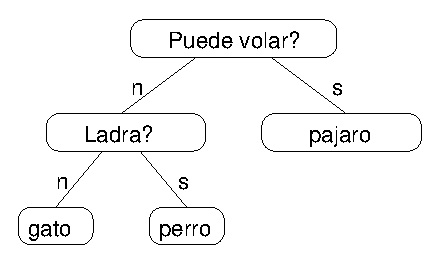
\includegraphics{illustrations/tree5}}
\afterfig

Al principio de cada ronda, el programa empieza en la raíz del árbol
y hace la primera pregunta. Dependiendo de la respuesta se mueve al
subárbol izquierdo o derecho y continúa hasta que llega a un nodo
hoja. En ese momento conjetura. Si falla, le pregunta al usuario el
nombre del animal y una pregunta que le permitiría distinguir el animal
conjeturado del real. Con esta información agrega un nodo al árbol
con la nueva pregunta y el nuevo animal.

Aquí está el código fuente:

\adjustpage{-2} %\pagebreak

\beforeverb 
\begin{pythoncode}
def animal():
  # Un solo nodo
  raiz = arbol("pajaro")

  # Hasta que el usuario salga
  while True:
    print
    if not si("Esta pensando en un animal? "): 
       break

    # Recorrer el arbol
    arbol = raiz
    while arbol.obtenerizquierdo() != None:
      pregunta = arbol.obtenercarga() + "? "
      if si(pregunta):
        arbol = arbol.obtenerderecho()
      else:
        arbol = arbol.obtenerizquierdo()

    # conjetura
    conjetura = arbol.obtenercarga()
    pregunta = "¿Es un" + conjetura + "? "
    if si(pregunta):
      print("¡Soy el mejor!")
      continue

    # obtener mas informacion
    pregunta  = "¿Cual es el nombre el animal? "
    animal  = input(pregunta)
    pregunta  = "¿Que pregunta permitiria 
                  distinguir un %s de un %s? "
    q = input(pregunta % (animal,conjetura))

    # agrega un nuevo nodo arbol
    arbol.asignarcarga(q)
    pregunta = "¿Si el animal fuera %s 
                la respuesta sería? "
    if si(pregunta % animal):
      arbol.asignarizquierdo(arbol(conjetura))
      árbol.asignarderecho(arbol(animal))
    else:
      arbol.asignarizquierdo(arbol(animal))
      arbol.asignarderecho(arbol(conjetura))
\end{pythoncode}
\afterverb La función \texttt{si} es auxiliar, imprime una pregunta
y recibe la respuesta del usuario. Si la respuesta empieza con {\em
s} o {\em S}, retorna cierto:

\beforeverb 
\begin{pythoncode}
def si(preg):
  from string import lower
  r = lower(input(preg))
  return (r[0] == 's')
\end{pythoncode}
\afterverb La condición del ciclo es \texttt{True}, lo que implica
que el ciclo iterará hasta que la sentencia \texttt{break} se ejecute
cuando el usuario deje de pensar en animales.

El ciclo \texttt{while} interno recorre el árbol desde la raíz hasta
el fondo, guiándose por las respuestas del usuario.

Cuando se agrega un nuevo nodo al árbol, la nueva pregunta reemplaza
la carga, y los dos hijos son el animal nuevo y la carga original.

Una limitación seria de este programa es que cuando finaliza, ¡olvida
todo lo que se le ha enseñado!
\begin{quote}
{\em Como ejercicio, piense en diferentes maneras de guardar este
árbol de conocimiento en un archivo. Implemente la que parezca más
sencilla.} 
\end{quote}

\section{Glosario}

\index{árbol binario} \index{nodo} \index{nodo raíz} \index{nodo hoja}
\index{nodo padre} \index{nodo hijo} \index{nodo hermano} \index{nivel}
\index{prefija} \index{preorden} \index{postorden} \index{en orden}
\index{operador binario} \index{operador!binario}
\begin{description}
\item [{Arbol binario:}] un árbol en el que cada nodo se refiere a cero,
uno o dos nodos, llamados hijos.
\item [{Raíz:}] nodo inicial en un árbol, es el único que no tiene padre.
\item [{Hoja:}] nodo que no tiene hijos y se encuentra lo mas abajo posible.
\item [{Padre:}] nodo que tiene la referencia hacia otro nodo.
\item [{Hijo:}] uno de los nodos referenciados por un nodo.
\item [{Hermanos:}] nodos que comparten un padre común.
\item [{Nivel:}] conjunto de nodos equidistantes a la raíz.
\item [{Operador binario:}] operador que acepta dos operandos.
\item [{Subexpresión:}] expresión en paréntesis que se puede ver como un
solo operando en una expresión más grande.
\item [{Preorden:}] es el recorrido sobre un árbol en el que se visita
cada nodo antes que a sus hijos.
\item [{Notación prefija:}] notación para escribir una expresión matemática
en la que cada operador aparece antes de sus operandos.
\item [{Postorden:}] forma de recorrer un árbol, visitando los hijos de
un nodo antes que a este.
\item [{En orden:}] forma de recorrer un árbol, visitando primero el subárbol
izquierdo, luego la raíz y por último, el subárbol derecho.
\end{description}

